\section{Muhammad Tomy 1174031}

\subsection{Teori}
\begin{enumerate}
\item Jelaskan apa itu random forest, sertakan gambar ilustrasi buatan sendiri.\par
Random Forest adalah konstruk data yang diterapkan pada machine learning yang mengembangkan sejumlah besar pohon keputusan acak yang menganalisis sekumpulan variabel. Jenis algoritma ini membantu meningkatkan cara teknologi menganalisis data yang kompleks. Juga merupakan algoritma machine learning yang fleksibel, mudah digunakan, bahkan tanpa penyetelan hyper-parameter, dengan hasil yang baik. Ini juga merupakan salah satu algoritma yang paling banyak digunakan, karena kesederhanaan dan faktanya dapat digunakan untuk tugas klasifikasi dan regresi.\\
Dibawah ini merupakan salah satu ilustrasi penggunaan Random Forest.
\begin{figure}[ht]
\centering
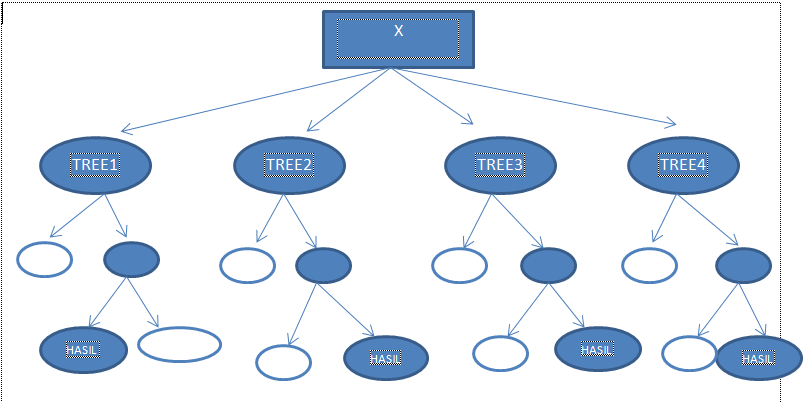
\includegraphics[scale=0.5]{figures/1174031/3/teori1.PNG}
\caption{Random Forest}
\label{contoh}
\end{figure}

\item Jelaskan cara membaca dataset khusus dan artikan makna setiap file dan isi field masing masing file.
Dataset adalah kumpulan data. Paling umum satu data set sesuai dengan isi tabel database tunggal, atau matriks data statistik tunggal, di mana setiap kolom tabel mewakili variabel tertentu, dan setiap baris sesuai dengan anggota tertentu dari dataset yang dipertanyakan.
\begin{itemize}
\item
Gunakan librari Pandas pada python untuk dapat membaca dataset dengan format text file.
\item
Setelah itu, buat variabel baru "dataset" yang berisikan perintah untuk membaca file csv.
\item
Memanggil Librari Panda untuk membaca dataset
\item
Membuat variabel "Dataset" yang berisikan pdreadcsv untuk membaca dataset. Pada contoh ini menggunakan txt tapi tetap bisa membaca datasetnya, mengapa? Karena pada saat dijalankan librari panda secara otomatis akan mengubah data dalam bentuk text file ke format csv.
\end{itemize}

\item Jelaskan apa itu Cross Validation.
Cross Validation adalah prosedur resampling yang digunakan untuk mengevaluasi model machine learning pada sampel data yang terbatas. Prosedur ini memiliki parameter tunggal yang disebut k yang mengacu pada jumlah grup tempat sampel data yang akan dibagi. Karena itu, prosedur ini sering disebut k-fold cross-validation.
Proses penentuan apakah hasil numerik yang mengukur hubungan yang dihipotesiskan antar variabel, dapat diterima sebagai deskripsi data, dikenal sebagai Validationi. Umumnya, estimasi kesalahan untuk model dibuat setelah training, lebih dikenal sebagai evaluasi residu. Dalam proses ini, estimasi numerik dari perbedaan respons yang diprediksi dan yang asli dilakukan, juga disebut kesalahan training. Namun, ini hanya memberi kita gambaran tentang seberapa baik model kita pada data yang digunakan untuk melatihnya. Sekarang mungkin bahwa model tersebut kurang cocok atau overfitting data. Jadi, masalah dengan teknik evaluasi ini adalah bahwa itu tidak memberikan indikasi seberapa baik pelajar akan menggeneralisasi ke set data independen / tidak terlihat. Model ini dikenal sebagai Cross Validation.

\item Jelaskan apa arti score 44 \% pada random forest, 27 \% pada decision tree dan 29 \% dari SVM.
Itu merupakan presentase keakurasian prediksi yang dilakukan pada saat testing menggunakan label pada dataset yang digunakan. Score merupakan mendefinisikan aturan evaluasi model. Maka pada saat dijalankan akan muncuk persentase tersebut yang menunjukan keakurasian atau keberhasilan dari prediksi yang dilakukan. Jika menggunakan Random Forest maka hasilnya 40\% , jika menggunakan Decission Tree hasil prediksinya yaitu 27\% dan pada SVM 29\% .

\item Jelaskan bagaimana cara membaca confusion matriks dan contohnya memakai gambar atau ilustrasi sendiri.
Perthitungan Confusion Matriks dapat dilakukan sebagai berikut. Disini saya menggunakan data yang dibuat sendiri untuk menampilkan data aktual dan prediksi.
\begin{itemize}
\item
Import librari Pandas, Matplotlib, dan Numpy.
\item
Buat variabel y actu yang berisikan data aktual.
\item
Buat variabel y pred berisikan data yang akan dijadikan sebagai prediksi.
\item
Buat variabel df confusion yang berisikan crosstab untuk membangun tabel tabulasi silang yang dapat menunjukkan frekuensi kemunculan kelompok data tertentu.
\item
Pada variabel df confusion definisikan lagi nama baris yaitu Actual dan kolomnya Predicted
\item
Kemudian definisikan suatu fungsi yang diberi nama plot confusion matrix yang berisikan pendefinisian confusion matrix dan juga akan di plotting.
\lstinputlisting{src/1174031/3/1.py}
\end{itemize}
\begin{figure}[ht]
\centering
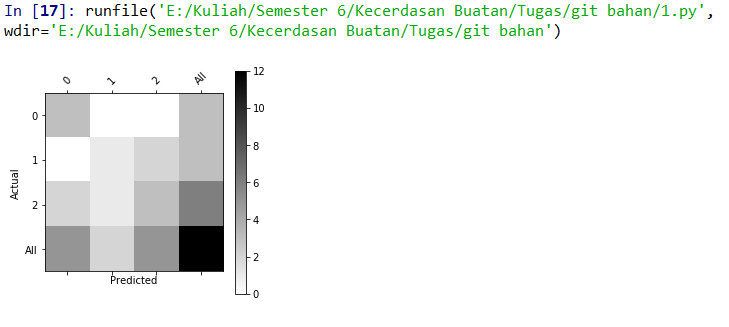
\includegraphics[scale=0.5]{figures/1174031/3/1.PNG}
\caption{Confusion Matriks}
\label{contoh}
\end{figure}

\item Jelaskan apa itu voting pada random forest disertai dengan ilustrasi gambar sendiri.\par
Voting yaitu suara untuk setiap target yang diprediksi pada saat melakukan Random Forest. Pertimbangkan target prediksi dengan voting tertinggi sebagai prediksi akhir dari algoritma random forest.
\begin{itemize}
\item
Untuk menggunakan Voting pada Random Forest dapat dilihat code berikut. Disini saya mengilustrasikan voting untuk berbagai macam algoritma terutama Random Forest.
\begin{figure}[ht]
\centering
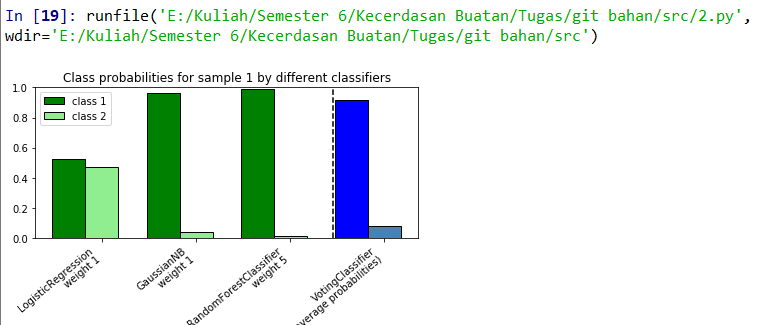
\includegraphics[scale=0.5]{figures/1174031/3/2.PNG}
\caption{Voting}
\label{contoh}
\end{figure}
\end{itemize}
\end{enumerate}


\subsection{Praktikum}
\begin{enumerate}
\item pandas \par
pada baris ke satu yaitu perintah mengimport library padas pada python atau anaconda kemudian di inisialisasikan menjadi karakter. selanjutnya ada sebuah array yang berisi a b c d. selanjutnya penggunaan array tipe series dan yang terakhir perintah print untuk menampilkan data pada karakter.
\lstinputlisting{src/1174031/3/3.py}
\begin{figure}[ht]
\centering
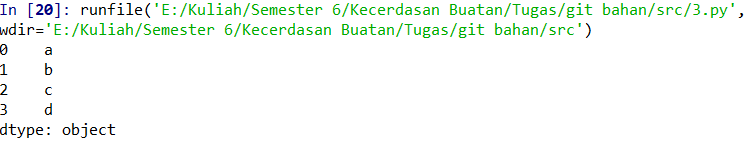
\includegraphics[scale=0.5]{figures/1174031/3/3.PNG}
\caption{hasil}
\label{contoh}
\end{figure}

\item numpy\par
Arti tiap baris codingan pada aplikasi sederhana numpy adalah sebagai berikut : pada baris ke satu yaitu mengimport numpy yang di inisialisasi menjadi np kemudian pada baris selanjutnya berisikan arange yang berarti membuat data yang berisi 12 dan ada reshape yang berfungsi merubah bentuk dari satu baris menjadi 2 baris data. Lalu yang terkhir ada perintah untuk print yaitu menampilkan data dari dika.
\lstinputlisting{src/1174031/3/4.py}
\begin{figure}[ht]
\centering
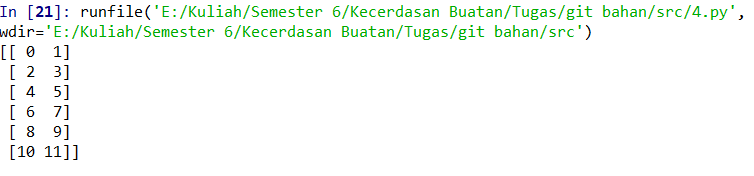
\includegraphics[scale=0.5]{figures/1174031/3/4.PNG}
\caption{hasil}
\label{contoh}
\end{figure}

\item matplotlib\par
Arti tiap baris aplikasi sederhana matplotlib pada baris ke satu yaitu memasukan library matplotlib.pyplot yang di definisikan menjadi plt kemudian plt.plot untuk menentukan grafik yang akan dibuat. lalu membuat variabel y dengan nama some number yang terakhir untuk menampilkan data pada sebuah grafik.
\lstinputlisting{src/1174031/3/5.py}
\begin{figure}[ht]
\centering
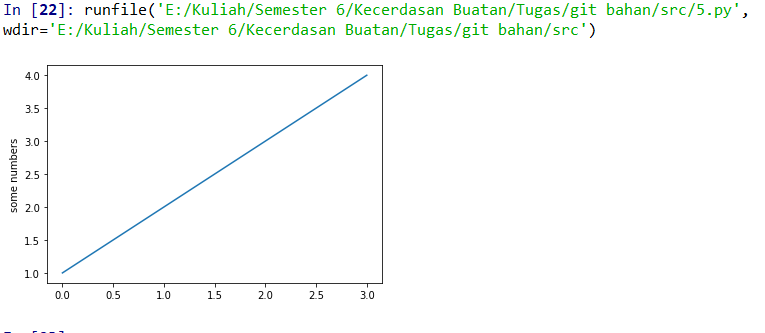
\includegraphics[scale=0.5]{figures/1174031/3/5.PNG}
\caption{hasil}
\label{contoh}
\end{figure}

\item Random Forest\par
Arti tiap baris hasil codingan random forest pada baris pertama random forest di import dari sklearn dengan ketentuan yaitu Nilai default untuk parameter yang mengontrol ukuran pohon (mis. Max\_depth, min\_samples\_leaf, dll.) Mengarah ke pohon yang tumbuh besar dan tidak di-unsuned yang berpotensi sangat besar pada beberapa set data. Untuk mengurangi konsumsi memori, kompleksitas dan ukuran pohon harus dikontrol dengan menetapkan nilai parameter tersebut.
\lstinputlisting{src/1174031/3/6.py}
\begin{figure}[ht]
\centering
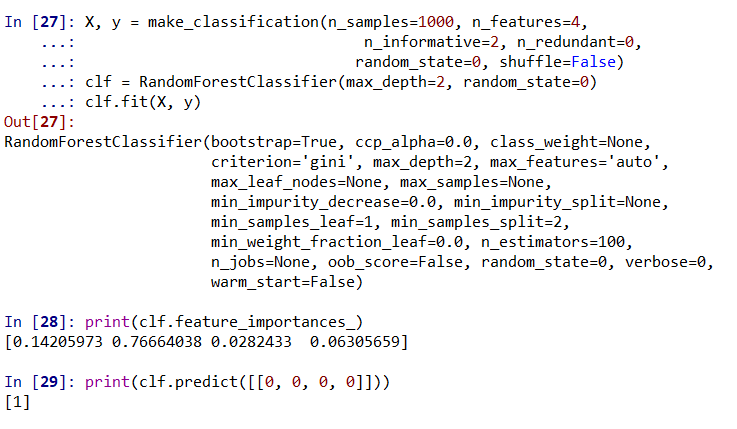
\includegraphics[scale=0.5]{figures/1174031/3/7.PNG}
\caption{hasil}
\label{contoh}
\end{figure}

\item Confusion Matrix\par
arti codingan pada hasil tiap codingan confusion matrix pada baris pertama codingan tersebut mendeskripsikan atau mengimport confusion matrix dari sklearn kemudian dibuat variabel y\_true untuk nilai target ground truth (benar). y\_pred untuk Taksiran target seperti yang dikembalikan oleh classifier. lalu menampilkan kedua variabel.
\lstinputlisting{src/1174031/3/7.py}
\begin{figure}[ht]
\centering
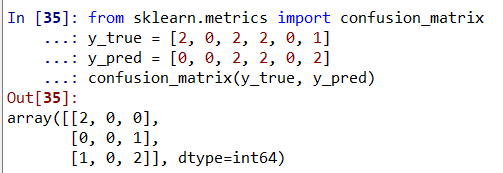
\includegraphics[scale=0.5]{figures/1174031/3/8.PNG}
\caption{hasil}
\label{contoh}
\end{figure}

\item SVM dan Decision Tree\par
Seperti pengklasifikasi lainnya, DecisionTreeClassifier mengambil input dua array: array X, jarang atau padat, dengan ukuran n\_samples, n\_features memegang sampel pelatihan, dan array Y dari nilai integer, ukuran n\_samples,Atau, probabilitas setiap kelas dapat diprediksi. Seperti pengklasifikasi lainnya, SVC, NuSVC dan LinearSVC mengambil input dua array: array X ukuran n\_samples, n\_features memegang sampel pelatihan, dan array y label kelas (string atau bilangan bulat), ukuran n\_samples:
\lstinputlisting{src/1174031/3/8.py}
\begin{figure}[ht]
\centering
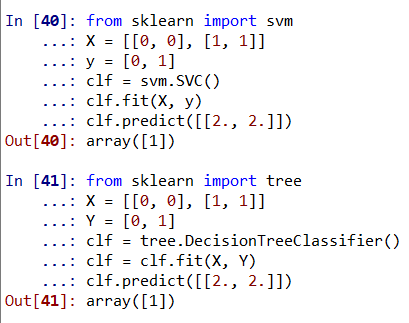
\includegraphics[scale=0.5]{figures/1174031/3/9.PNG}
\caption{hasil}
\label{contoh}
\end{figure}

\item Cross Validation\par
 digunakan untuk memeriksa akurasi dari ketepatan hasil pengolahan data tersebut maka akan didapat nilai rata-rata 60 persen dari hasil pengolahan data tersebut untuk lebih jelasnya dapat di lihat pada gambar pada codingan tersebut pada baris ke satu melakukan import library dari sklern kemudian pada baris selanjutnya mengisi nilai skor dengan nilai pada variabel lontong setelah hal tersebut dilakukan kemudian data tersebut di eksekusi. berikut merupakan hasil dari code tersebut dapat dilihat pada gambar.
\lstinputlisting{src/1174031/3/9.py}
\begin{figure}[ht]
\centering
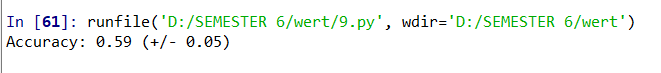
\includegraphics[scale=0.5]{figures/1174031/3/10.PNG}
\caption{hasil}
\label{contoh}
\end{figure}

\item program pengamatan
arti dari hasil program pengamatan. perogram pengamatan dapat mengamati dari 3 aspek diatas yaitu svm, random, dan decision tree. Yang memiliki variabel X Y Z dan di tampilkan dalam bentuk grafik. 
\lstinputlisting{src/1174031/3/10.py}
\begin{figure}[ht]
\centering
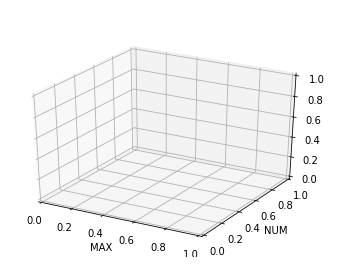
\includegraphics[scale=0.5]{figures/1174031/3/11.PNG}
\caption{hasil}
\label{contoh}
\end{figure}
\end{enumerate}


\subsection{Penanganan Error}
Screenshot error
\begin{enumerate}
\item  Untuk gambar screenshot error
\begin{figure}[ht]
\centering
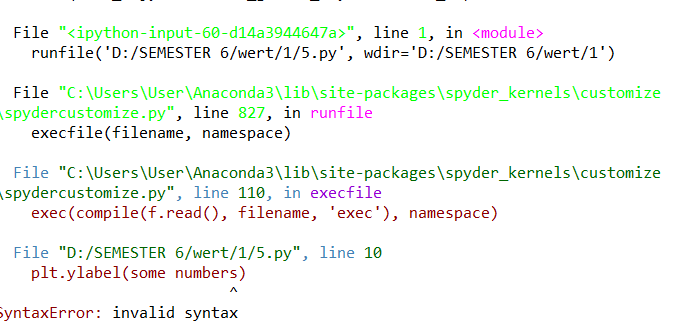
\includegraphics[scale=0.5]{figures/1174031/3/error.PNG}
\caption{hasil}
\label{contoh}
\end{figure}
\end{enumerate}

Code Errornya 
\begin{verbatim}
import matplotlib.pyplot as plt
plt.plot([1, 2, 3, 4])
plt.ylabel(some numbers)
plt.show()
\end{verbatim}
\par
pada kode ylabel memiliki nama atau isi some numbers tetapi pada tipe data tertentu harus di awali dan diakhiri dengan tanda petik 2 atau 1. Pada kodingnya hanya kurang tanda petik 1.

